\documentclass[openany,12pt]{book}
\usepackage[utf8]{inputenc}
\usepackage{etoolbox}
\usepackage{hyperref}
\usepackage{geometry}
\usepackage{titlesec}
\usepackage{fancyhdr}

\usepackage{xr-hyper} % External referencing
% \externaldocument[func:]{../Functions/functions} % Path to functions.aux


\usepackage{colortbl}
\usepackage{graphicx}
\usepackage{float}

\usepackage{soul}

\usepackage{enumitem}


\usepackage{array}
\usepackage{booktabs}

\usepackage{listings}
\lstset{
    language=C++,
    basicstyle=\ttfamily\footnotesize,     % the size of the fonts used for the code
    keywordstyle=\color{blue}\bfseries,    % keywords
    ndkeywordstyle=\color{magenta},        % more keywords like types (int, char, etc.)
    identifierstyle=\color{black},         % variable names
    commentstyle=\color{gray}\itshape,     % comments
    stringstyle=\color{teal},              % strings
    numberstyle=\tiny\color{gray},         % line numbers
    numbers=left,                          % line number position
    numbersep=8pt,                         % distance of line numbers from code
    backgroundcolor=\color{white},         % background color
    showspaces=false,                      % show spaces (only for debugging)
    showstringspaces=false,                % underline spaces in strings?
    showtabs=false,                        % show tabs (only for debugging)
    tabsize=4,                             % tab space width
    breaklines=true,                       % automatic line breaking
    breakatwhitespace=true,                % only break at whitespace
    % frame=lines,                           % draw a frame at the top and bottom
    captionpos=b,                          % caption position
    escapeinside={(*@}{@*)},               % for LaTeX escapes
    morekeywords={nullptr, size_t, uint32_t, int32_t, override, final, constexpr, noexcept},
    columns=fullflexible,                  % better alignment
    keepspaces=true                        % keep spaces in text, useful for indentation
}




\usepackage{amsthm}
\usepackage{amsmath}

\newcommand{\code}[1]{\texttt{#1}}

\usepackage[dvipsnames]{xcolor}
\newcommand{\red}[1]{\textcolor{Red}{#1}}
\newcommand{\blue}[1]{\textcolor{RoyalBlue}{#1}}
\newcommand{\gray}[1]{\textcolor{gray}{#1}}
\newcommand{\green}[1]{\textcolor{Green}{#1}}
\newcommand{\purple}[1]{\textcolor{Purple}{#1}}
\newcommand{\orange}[1]{\textcolor{BurntOrange}{#1}}



% =====================================================
% ============== Listings Formats =====================






\geometry{margin=1in}
\titleformat{\section}{\large\bfseries}{\thesection}{1em}{}
\pagestyle{fancy}
\fancyhead[L]{Course Summary}
\fancyhead[C]{Operating Systems 234123}
\fancyhead[R]{Spring 2025}



% =====================================================
% =====================================================
% =====================================================
% % Define new counters
% \newcounter{lecture}
% \newcounter{tutorial}

% % Format titles to look like chapters
% \titleformat{\chapter}[display]
%   {\normalfont\Huge\bfseries}{\chaptername\ \thechapter}{20pt}{\Huge}

% \newcommand{\lecturechaptername}{Lecture}
% \newcommand{\tutorialchaptername}{Tutorial}

% % Custom "Lecture Chapter"
% \newcommand{\lecture}[1]{%
%   \clearpage
%   \refstepcounter{lecture}
%   \renewcommand{\chaptername}{\lecturechaptername}%
%   \addcontentsline{toc}{chapter}{Lecture \thelecture: #1}
%   \chapter*{Lecture \thelecture: #1}
%   \markboth{Lecture \thelecture}{#1}
% }

% % Custom "Tutorial Chapter"
% \newcommand{\tutorial}[1]{%
%   \clearpage
%   \refstepcounter{tutorial}
%   \renewcommand{\chaptername}{\tutorialchaptername}%
%   \addcontentsline{toc}{chapter}{Tutorial \thetutorial: #1}
%   \chapter*{Tutorial \thetutorial: #1}
%   \markboth{Tutorial \thetutorial}{#1}
% }


\newcounter{Topic}

% Format titles to look like chapters
\titleformat{\chapter}[display]
  {\normalfont\Huge\bfseries}{\chaptername\ \thechapter}{20pt}{\Huge}

\newcommand{\topicchaptername}{Topic}

% Custom "Topic Chapter"
\newcommand{\Topic}[1]{%
  \clearpage
  \refstepcounter{Topic}
  \renewcommand{\chaptername}{\topicchaptername}%
  \addcontentsline{toc}{chapter}{\topicchaptername\ \theTopic: #1}
  \chapter*{Topic \theTopic: #1}
  \markboth{Topic\theTopic}{#1}
}
% =====================================================
% =====================================================
% =====================================================

\title{Operating Systems (02340123)\\ Summary - Spring 2025}
\author{Razi \& Yara}
\date{\today}

\begin{document}

\maketitle
\tableofcontents
\newpage



% ====================================================
% ====================================================
% ====================================================
% ------------------- Notes Section ------------------
% ====================================================
% ====================================================
% ====================================================

\part{Lectures \& Tutorials}



% =====================================================
% ================== Lecture 1 ========================
% =====================================================

\Topic{Introduction}

\paragraph{Operating System (OS)}%
An Operating System's job is:
\begin{itemize}
    \item Coordinate the execution of all SW, mainly user apps.
    \item Provide various common services needed by users \& apps.
    \item An OS of a physical server controls its physical devices, e.g. CPU, memory, disks, etc.
    \item An OS of a virtual server only \textit{believes} it does. There's another OS underneath, called \textbf{hypervisor} which fakes it.
\end{itemize}

\vspace{1em}
\noindent Using an OS allows us to take advantage of \textbf{\textit{"virtualization"}}:
\begin{itemize}
    \item \textbf{Server Consolidation:} Run multiple servers on one physical server. This is allows for better resource utilization, smaller spaces, and less power consumption.
    \item \textbf{Disentangling SW from HW:} allows for backing up/restoring, live migration, and HW upgrade. This give us the advantage of easier provisioning of new (virtual) servers = "virtual machines", and easier OS-level development and testing.
\end{itemize}

\vspace{1em}
Most importantly, an OS is \textbf{reactive}, "event-driven" system, which means it waits for events to happen and then reacts to them. This is in contrast to typical programs which run from start to end without waiting for external events to occur to invoke them.

\begin{center}
    \rowcolors{2}{gray!15}{white}
    \begin{tabular}{|>{\raggedright\arraybackslash}p{4.5cm}
        |>{\raggedright\arraybackslash}p{6.5cm}
        |>{\raggedright\arraybackslash}p{5.5cm}|}
        \hline
        \rowcolor{blue!30}
         & \textbf{Typical Programs}                                                    & \textbf{OS} \\
        \hline
        \textbf{What does it typically do?}
         & Get some input, do some processing, produce output, terminate
         & Waits \& reacts to ``events''                                                              \\
        \hline
        \textbf{Structure}
         & Has a \texttt{main} function, which is (more or less) the entry point
         & No \texttt{main}; multiple entry points, one per event                                     \\
        \hline
        \textbf{Termination}
         & End of \texttt{main}
         & Power shutdown                                                                             \\
        \hline
        \textbf{Typical goal}
         & $\sim$ Finish as soon as possible
         & Handle events as quickly as possible $\Rightarrow$ more time for apps to run               \\
        \hline
    \end{tabular}
\end{center}

\paragraph{Event Synchronousation} OS events can be classified into two:
\begin{itemize}
    \item \textbf{Asynchronous interrupts:} keyboard, mouse, network, disk, etc. These are events that can happen at any time and the OS must be ready to handle them.
    \item \textbf{Synchronous:} system calls, divide by zero, page faults, etc. These are events that happen as a result of the program's execution and the OS must handle them immediately.
\end{itemize}


\paragraph{Multiplexing}
Multiplexing is the ability of an OS to share a single resource (e.g. CPU, memory, disk) among multiple processes or threads. This allows for better utilization of resources and enables multiple applications to run concurrently.
*Multiprogramming  means multiplexing the CPU recourse.


Notable services provided by an OS:
\begin{enumerate}
    \item \textbf{Isolation:} Allow multiple processes to coexist using the same resources without stepping on each other's toes.
          Usually achieved by multiplexing the CPU, memory, and other resource done by the OS. However, some physical resources know how to multiplex themselves, e.g. network cards, sometimes called \textit{"self-virtualizing devices"}.
    \item \textbf{Abstraction:} Provides convenience \& portability by:
          \begin{itemize}
              \item offering more meaningful, higher-level interfaces
              \item hiding HW details, making interaction wiht HW easier.
          \end{itemize}
\end{enumerate}



% =====================================================
% ================== Lecture 2 ========================
% =====================================================

\Topic{Processes \& Signals}
\section*{Processes}

\begin{center}
    \begin{minipage}[t]{0.6\textwidth}
        \vspace{0pt} % force top alignment
        Each process is an instance of a program in execution, which includes:
        \begin{itemize}
            \item \textbf{Program code:} The actual code of the program.
            \item \textbf{Process state:} The current state of the process, including the program counter, registers, and memory management information.
            \item \textbf{Process control block (PCB):} A data structure used by the OS to manage the process, containing information such as process ID, process state, CPU registers, memory management information, and I/O status information.

                  A process \ul{doesn't have direct access to its PCB}, it is managed by the OS (kernel space), i.e. needs privilege level 0 (kernel mode) to access it.

                  Each PCB contains: \code{real\_parent}, \code{parent}, \code{children}, \code{siblings},...\\
                  Each process has a \code{task\_struct current} pointer to its PCB.

            \item \textbf{Process ID (PID):} A unique identifier assigned to each process by the OS. The PID is used by the OS to manage the process and is used in system calls to refer to the process.
        \end{itemize}
    \end{minipage}%
    \hspace{1em}
    \begin{minipage}[t]{0.35\textwidth}
        \vspace{0pt} % force top alignment
        \centering
        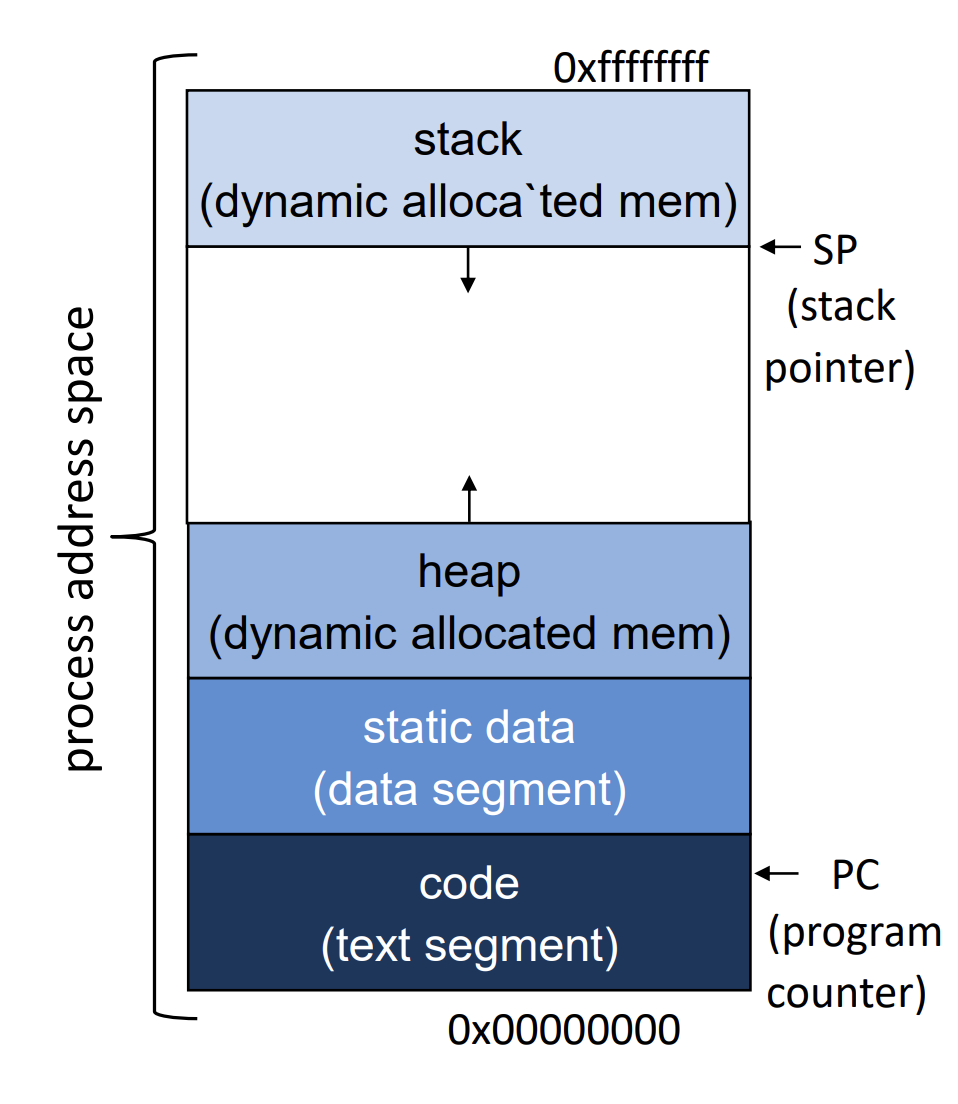
\includegraphics[width=\linewidth]{../Assets/process_memory.png}
    \end{minipage}
\end{center}



\paragraph{Process States}
A process can be in one of the following states:
\begin{itemize}
    \item \textbf{Running:} The process is currently being executed by the CPU.
    \item \textbf{Ready:} The process is ready to be executed but is waiting for the CPU to become available.
    \item \textbf{Waiting:} The process is waiting for an event to occur, such as I/O completion or a signal.
    \item \textbf{Zombie:} The process has terminated but its PCB is still in the system, waiting for the parent process to read its exit status. In this state, the process has released almost all of its resources, but \blue{the PCB is still in the system}.
\end{itemize}



\begin{figure}
    \centering
    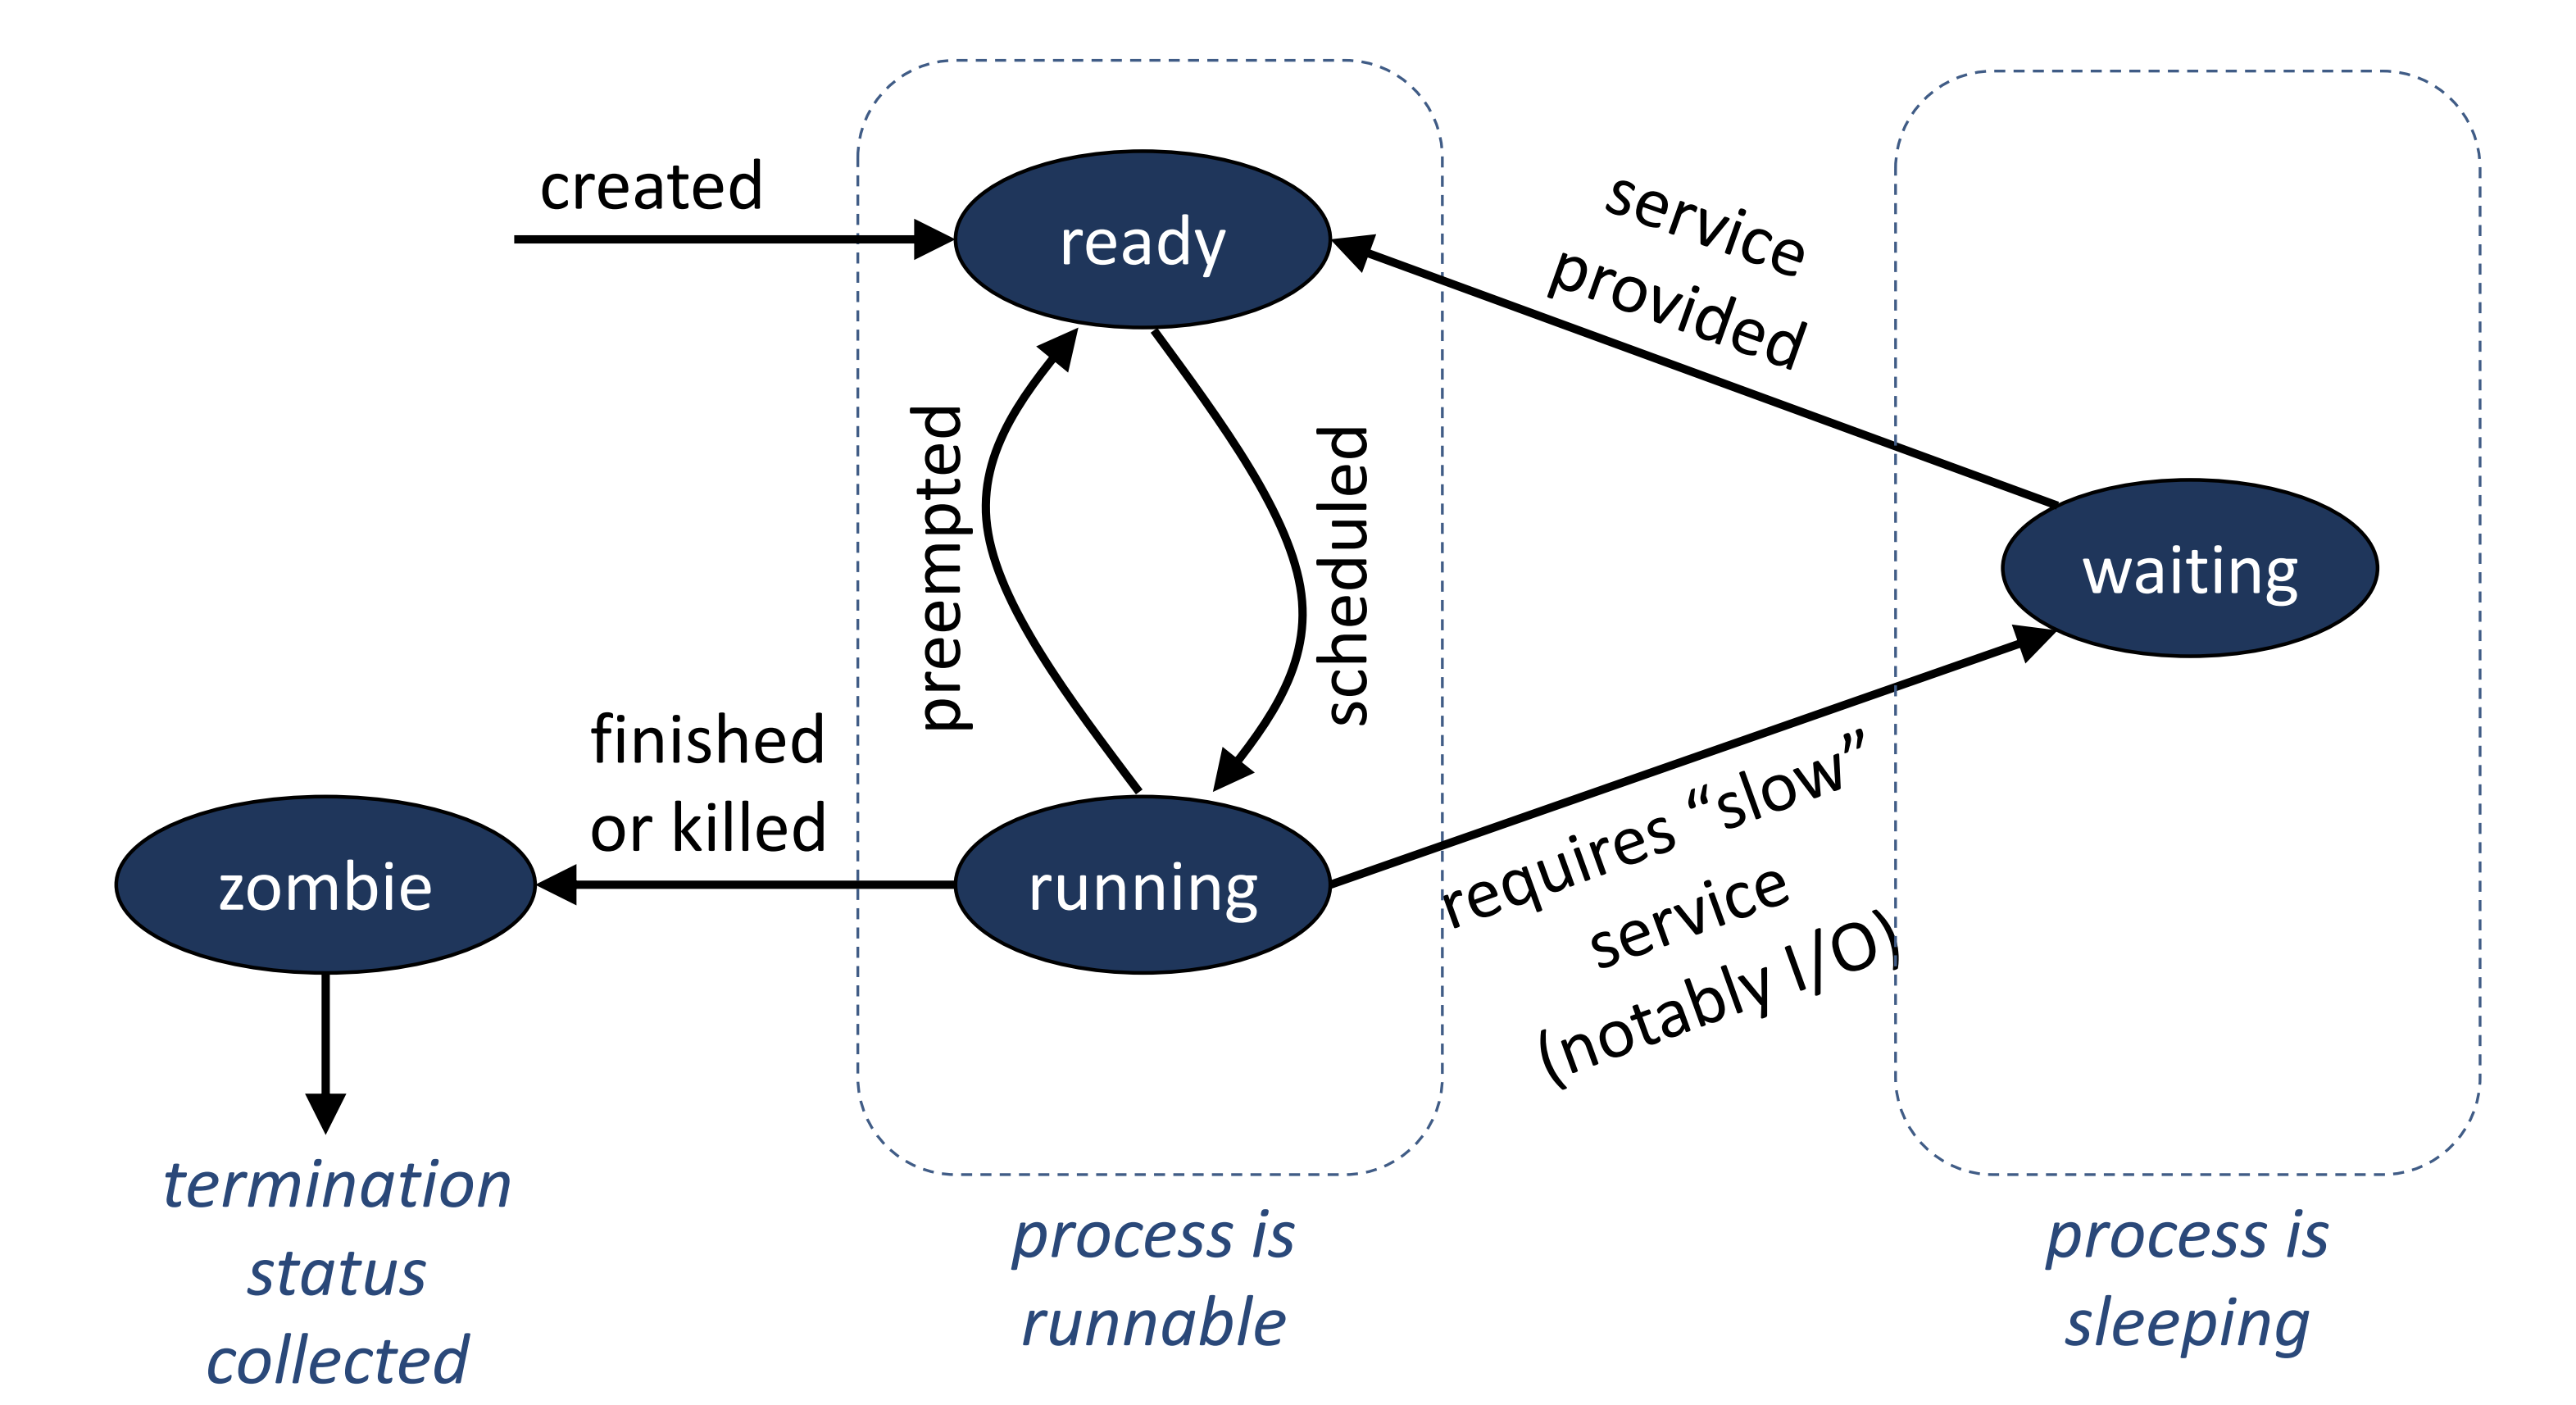
\includegraphics[width=0.8\textwidth]{../Assets/process_states.png}
    \caption{Process States}
    \label{fig:process_states}
\end{figure}


As we saw in "ATAM", each process can only access a certain set of utilites and functions, those who require privilege level 3 (user mode). So to access the OS services, a process must use \textbf{system calls} which are functions provided by the OS that allow processes to request services from the OS. System calls are typically implemented in the OS kernel and provide a controlled interface for processes to interact with the OS.

\vspace{1em}

Each \textit{syscall}, in case of an error, will change the \texttt{errno} variable to indicate the error type. The \texttt{errno} variable is a global variable that is set by system calls and some library functions in the event of an error to indicate what went wrong. It is defined in the header file \texttt{errno.h}. {\color{blue}\textbf{Note:} \texttt{errno} is not reset to 0 after a successful syscall, so it must be checked immediately after the syscall, and be reset before usage if need be} (if there is not any other way to make sure there is an error indeed).\\
i.e. \code{errno = <Number of Last Syscall Error>;}

\vspace{1em}

As noted above, each process must be \code{wait()}ed for by its parent process to be able to release its PCB and resources. This is done by the \texttt{wait()} syscall, which suspends the calling process until one of its children terminates. In case {\color{red} the parent process terminates before the child}, the child process {\color{red} becomes an orphan process and is adopted by the init process (PID 1)}, which will then wait for it to terminate and release its resources.


\paragraph{Process Management} The OS offers various system calls to manage processes, including: \gray{(More details in the functions reference)}
\begin{itemize}
    \item \texttt{fork()}: Creates a new process by duplicating the calling process. The new process is called the child process, and the calling process is called the parent process.
    \item \texttt{exec()}: Replaces the current process image with a new process image, effectively running a different program in the same process.
    \item \texttt{wait()}: Suspends the calling process until one of its children terminates.
    \item \texttt{exit()}: Terminates the calling process and releases its resources.
    \item \texttt{getpid()}: Returns the process ID of the calling process.
    \item \texttt{getppid()}: Returns the process ID of the parent process.
    \item \texttt{kill()}: Sends a signal to a process, which can be used to terminate or suspend the process.
\end{itemize}

\paragraph{Parent Vs. Real Parent Process}
The real parent process is the one that created the current process using \code{fork()}, or the one that adopted it in case the real parent terminated before the child.

The parent process is the one \textit{tracing} the current process, e.g. using \code{ptrace()}. The parent process is the one that will receive signals from the current process, e.g. \texttt{SIGCHLD} when the current process terminates.

In most cases, the parent process is the real parent process, but it can be different in some cases, e.g. when a process is being traced by a debugger.



\paragraph{Daemon Processes}
A daemon process is a background process not controlled by the user.
To run a process as a daemon use \code{nohup <command> \&}.

Daemon names usually end with the letter "d", e.g. \texttt{sshd} (SSH daemon), \texttt{httpd} (HTTP daemon), etc.




% ===================================================== Signals Section
\newpage
\section*{Signals}
\paragraph{Signals}
Signals are "notifications" sent to a process to asynchronously notify it that some event has occurred.

* Receiving a signal only occurs then returning from kernel mode, which in turn invokes the corresponding signal handler.

** Default signal handling actions: Either die or ignore

*** In case of several signals from different types, they will be handled by the order of their definition in the signals register.


\vspace{1em}

Each signal has a name, a number, and a default action. All but 3 signals can be blocked, i.e. ignored until the process is ready to handle them. The 3 signals that cannot be blocked are:
\begin{itemize}
    \item \texttt{SIGKILL}: Used to forcefully terminate a process. (Process becomes a zombie)
    \item \texttt{SIGSTOP}: Used to suspend the receiving process. (Make it sleep) The signals is sent when the user presses Ctrl+Z in the terminal. {\color{gray}Note: In truth Ctrl+Z sends the \texttt{SIGTSTP} signal, however, we don't learn about the differences between the two signals in this course.}
    \item \texttt{SIGCONT}: Used to resume a suspended process, usually sent after a \texttt{SIGSTOP} signal. The handler for this signal can be customized but it {\color{red}will always} resume the process.
\end{itemize}
\texttt{SIGSTOP} and \texttt{SIGCONT} are useful for debugging purposes, allowing the user to pause and resume the execution of a process.

\paragraph{Signal Handling}
A process can define a custom signal handler for a specific signal using the \texttt{signal()} or \texttt{sigaction()} {\color{gray}preferred} system calls.
To ignore a signal, the process can set its handler to \texttt{SIG\_IGN}. To restore the default action for a signal, the process can set its handler to \texttt{SIG\_DFLT}.

\paragraph{Signal Masking}
A process can block signals using the \texttt{sigprocmask()} system call, which allows the process to specify a set of signals to block. This is allows the process to overcome \textit{Race Conditions} resulted from the asynchronous nature of signals.\\
\indent This is achieved by maintaining a set of currently blocked signals \& a set of masked signals which is saved in the {\color{blue}PCB}.\\
\texttt{Blocked Signals} = mask array.\\
\texttt{Pending Signals} = signals that were sent to the process while it was blocked, and will be handled when the process unblocks them.

\newpage
\paragraph{Common Signals} the following are some of the most common signals:
\begin{enumerate}
    \item \textbf{\code{SIGSEGV, SIGBUS, SIGIILL, SIGFPE}}: These are driven by the associated \blue{(HW) interrupts} - The OS gets the associated interrupt, then the OS interrupt handler sees to it that the misbehaving process gets the associated signal, lastly the signaly handler is invoked.
          \begin{itemize}
              \item \texttt{SIGSEGV}: Segmentation violation (illegal memory reference, e.g., outside an array).
              \item \texttt{SIGBUS}: Dereference invalid address (null/misaligned, assume it's like SEGV).
              \item \texttt{SIGIILL}: Illegal instruction (trying to invoke privileged instruction).
              \item \texttt{SIGFPE}: Floating-point exception (despite the name, \textit{all} arithmetic errors, not just floating point. e.g., division by zero).
          \end{itemize}

    \item \textbf{\code{SIGCHLD}}: Parent \gray(not real parent) get it whenver \code{fork()}ed child terminates or is \code{SIGSTOP}-ed.

    \item \textbf{\code{SIGALRM}}: Get a signal after some specified time, can be set using the \blue{\code{alarm()} \& \code{setitimer()}} system calls.

    \item \textbf{\code{SIGTRAP}}: When debuggin/single-stepping a process, the debugger can set a breakpoint in the code, which will cause the process to receive a \texttt{SIGTRAP} signal when it reaches that point.

    \item \textbf{\code{SIGUSR1, SIGUSR2}}: User-defined signals, user can decide the meaning of these signals and their handlers.

    \item \textbf{\code{SIGPIPE}}: Write to pipe with no readers.

    \item \textbf{\code{SIGINT}}: Sent when the user presses Ctrl+C in the terminal. The default action is to terminate the process, but it can be customized.

    \item \textbf{\code{SIGXCPU}}: Delivered when a process used up more CPU than its soft-limit allows: soft/hard limits are set using the \blue{\code{setrlimit()}} system call. Soft-limits warn the process its about to exceed the hard-limit, Exceeding the hard-limit will cause \code{SIGKILL} to be sent to the process.

    \item \textbf{\code{SIGIO}}: Can configure file descriptors such that a signal will be delivered whenever some I/O is ready.

          Typically makes sense when also configuring the file descriptor to be \textit{non-blocking}, e.g., when \code{read()}ing from a non-blocking file descriptor, the system call immediately returns to user if there's currently nothing to read. In this case, \code{errno} will be set to \code{EAGAIN=EWOULDBLOCK}.
\end{enumerate}


\begin{samepage}
    \begin{center}
        \textbf{Signals Vs. Interrupts}
        \rowcolors{2}{gray!15}{white}
        \begin{tabular}{|>{\raggedright\arraybackslash}p{4.5cm}|>{\raggedright\arraybackslash}p{5.5cm}|>{\raggedright\arraybackslash}p{5.5cm}|}
            \hline
            \rowcolor{blue!30}
             & \textbf{interrupts}                                                                      & \textbf{signals} \\
            \hline
            Who triggers them? \newline Who defines their meaning?
             & Hardware: \newline CPU cores (sync) \& other devices (async)
             & Software (OS), \newline HW is unaware                                                                       \\
            \hline
            Who handles them? \newline Who (un)blocks them?
             & OS
             & processes                                                                                                   \\
            \hline
            When do they occur?
             & Both synchronously \& asynchronously
             & Likewise, but, technically, \newline invoked when returning \newline from kernel to user                    \\
            \hline
        \end{tabular}
    \end{center}
\end{samepage}





% =====================================================
% ================== Lecture 3 ========================
% =====================================================
\Topic{IPC - Inter-Process Communication}

\section*{Threads \& IPC}


\paragraph{Multiprocessing}
Using several CPU cores (=processors) for running a single job to solve a single "problem".


\begin{center}
    \begin{minipage}{0.45\textwidth}
        \vspace{0pt} % force top alignment
        \centering
        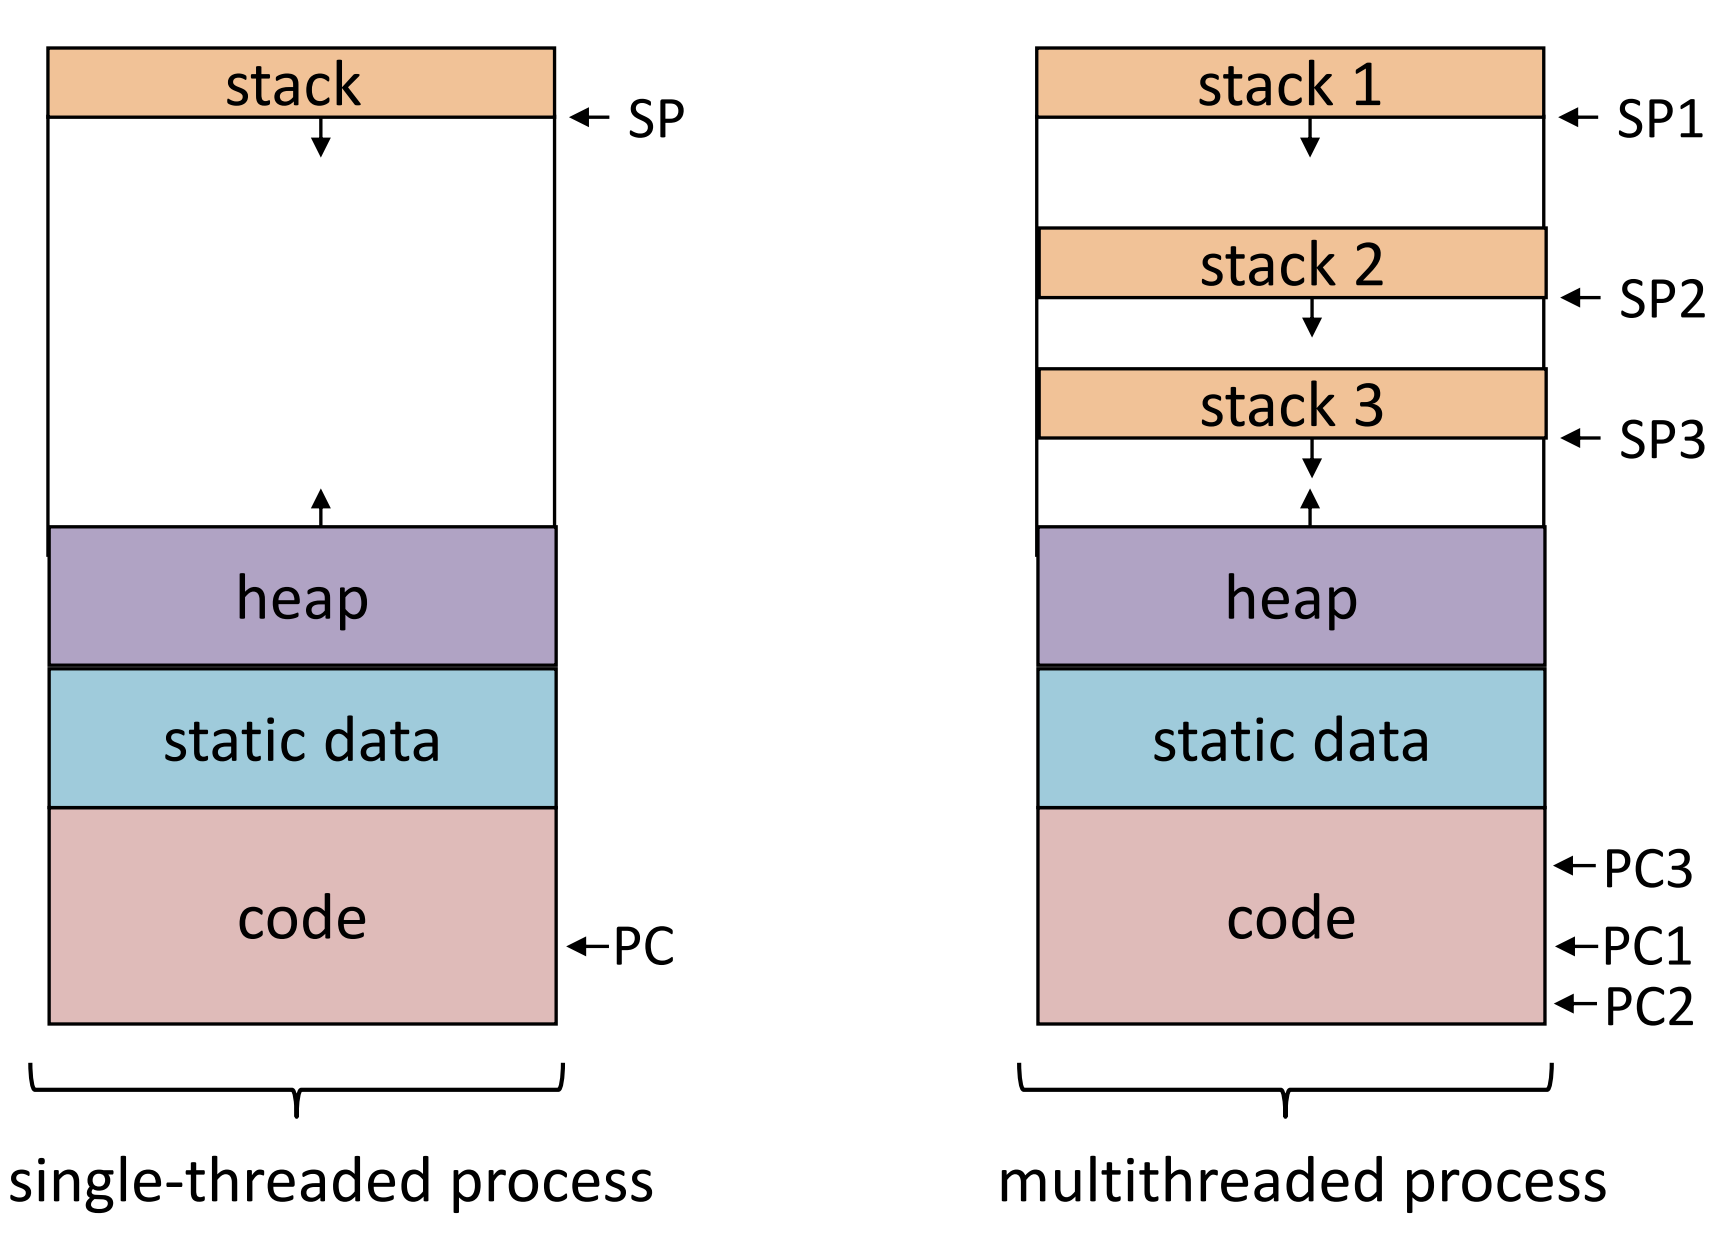
\includegraphics[width=\linewidth]{../Assets/thread_stack.png}
    \end{minipage}\hfill
    \begin{minipage}{0.5\textwidth}
        \vspace{0pt} % force top alignment  
        \paragraph{Threads}
        A process can have multiple threads, which share (nearly) everything, including the process's memory space, file descriptors, heap, static data, code segment and more.

        \hspace*{2em}However, each thread has its own stack, registers, and program counter. But they can still access each other's stack since they share the same memory space.
    \end{minipage}
\end{center}

Note that \blue{\textit{Global/Static Variables \& Dynamically Allocated Memory}} are shared between threads since they are stored in the Static Data Segment and the Heap, respectively, which are shared between all threads of a process. However, \red{\textit{Local Variables}} are not shared between threads since they are stored in the stack, which is unique to each thread.


\begin{samepage}
    \begin{center}
        \rowcolors{2}{gray!15}{white}
        \begin{tabular}{|>{\raggedright\arraybackslash}p{6cm}|
            >{\centering\arraybackslash}p{4cm}|
            >{\centering\arraybackslash}p{4cm}|}
            \hline
            \rowcolor{blue!30}
                                             & \textbf{Unique to Process} & \textbf{Unique to pthread} \\
            \hline
            Registers (notably PC)           & Y                          & Y                          \\
            Execution stack                  & Y                          & Y                          \\
            Memory address space             & Y                          & \red{N}                    \\
            Open files                       & Y                          & \red{N}                    \\
            Per-open-file position (=offset) & Y                          & \red{N}                    \\
            Working directory                & Y                          & \red{N}                    \\
            User/group credentials           & Y                          & \red{N}                    \\
            Signal handling                  & Y                          & \red{N}                    \\
            \hline
        \end{tabular}
    \end{center}
\end{samepage}


\newpage
\paragraph{OpenMP} Open Multi-Processing (OpenMP) consists of a set of compiler \textit{'pragma'} directives that allows the compiler to generate multi-threaded code for parallel execution.

\begin{center}
    \begin{minipage}{0.9\textwidth}
        \begin{lstlisting}
    #pragma omp parallel for
    for (i = 0; i < N; i++) {
            arr[i] = 2*i;
    } \end{lstlisting}
    \end{minipage}
\end{center}


\paragraph{Pthreads} POSIX threads (pthreads) is a standard for multi-threading in C/C++. It provides a set of functions to create and manage threads, as well as to synchronize them. \gray{(More details in the functions reference)}



\paragraph{File Descriptors} A non-negative integer representing an I/O "channel" on some device. File descriptors are saved in the process's \code{PCB} inside the \code{FDT} (File Descriptor Table), which is an array of pointers to \textit{file objects}, each representing an open file or device. So in fact, an FD is an index to a kernel array of channels.

Processes \red{don't} share \code{PCB} nor \code{FDT} but they \blue{can share file descriptors}, i.e. two processes can have the same file descriptor pointing to the same file object, which allows them to share the same open file or device. Upon forking, the child process inherits a copy of the parent's \code{FDT}. \blue{Note:} Threads \blue{do} share the same \code{FDT}.



\paragraph{Pipes} A pipe is a unidirectional communication channel between two processes, allowing one process to send data to another. Pipes are a pair of two file descriptors \code{int pipe\_fd[2]}. Each integer is a handle to a kernel communication object, \ul{which is a buffer that holds the data being sent between the two processes}.
\begin{itemize}
    \item \code{pipe\_fd[0]} = read side of the communication channel.
    \item \code{pipe\_fd[1]} = write side of the communication channel.
    \item Everything written via \code{pipe\_fd[1]} can be read via \code{pipe\_fd[0]}.
    \item \red{Blocking}: If the read side is empty, the read operation will block until data is written to the write side. If the write side is full, the write operation will block until space is available.
    \item \red{\code{SIGPIPE}}: Writing to a pipe whose read end is \code{close()}d will result in a \code{SIGPIPE} signal.
\end{itemize}



\begin{samepage}
    \begin{center}
        \rowcolors{2}{gray!15}{white}
        \begin{tabular}{|>{\raggedright\arraybackslash}p{4cm}|
            >{\raggedright\arraybackslash}p{6cm}|
            >{\raggedright\arraybackslash}p{5cm}|}
            \hline
            \rowcolor{blue!30}
            \textbf{Multi-tasking} & \textbf{Multi-programming} & \textbf{Multi-processing} \\
            \hline
            Having multiple processes \textit{time slice} on the same CPU core.
                                   &
            Having \textit{multiple jobs} in the system (either on the same core or on different cores). \gray{i.e. the existence of multiple processes in the system, regardless of whether they are running on the same core or not.}
                                   &
            Using \textit{multiple processors (CPU cores) for the same job} in parallel. \gray{i.e. creating multiple threads to run on different cores for the same process.}
            \\
            \hline
        \end{tabular}
    \end{center}
\end{samepage}





\newpage
\section*{Intro. Context Switching \& Caching}
\paragraph{Context Switching} is the process of saving the state of a currently running process and restoring the state of another process to allow it to run. This is done by the OS kernel and is necessary for multitasking, allowing multiple processes to share the CPU.
\begin{itemize}
    \item \textbf{Context} = the state of a process, including its registers, program counter, stack pointer, and memory management information.
    \item \textbf{Context Switch} = the process of saving the context of the currently running process and restoring the context of another process.
\end{itemize}

\paragraph{Context Switch Overhead} consists of two components:
\begin{itemize}
    \item \textbf{Direct Overhead:} The measurable time it takes to perform the context switch, which includes saving the current process's state and restoring the next process's state.
    \item \textbf{Indirect Overhead:} The time it takes for the CPU to cache the new process's data, which can be significant if the new process's data is not already in the CPU cache.
\end{itemize}

\paragraph{Cashing} The CPU cache is a small, fast memory that stores frequently accessed data to speed up access times. The Cache allows the CPU access to a fast memory that is closer to the CPU than the main memory (DRAM), and a larger one than the CPU registers. The cache works because of the \blue{\textit{Principle of Locality}}:
\begin{itemize}
    \item \textbf{Temporal Locality:} If at one point in time a particular memory location is referenced, then it is likely that the same location will be referenced again soon.
    \item \textbf{Spatial Locality:} If a particular memory location is referenced at a particular time, then it is likely that nearby memory locations will be referenced soon.
\end{itemize}



\paragraph{Copy-on-Write (COW)} The \code{fork()} system call creates a copy of the address space of the parent, but:
\begin{itemize}
    \item It only creates a \textit{logical} copy.
    \item There is no physical duplication of the memory pages, until we really need to write to them (from either process). And even then, only the page that is being written to is duplicated. \gray{(More details in the virutal memory lectures)}
\end{itemize}


\paragraph{User Level Threads (ULTs)} are threads that are managed by the user-level library, rather than the OS kernel. ULTs are not visible to the OS, which means that the OS does not know about them and does not schedule them. This allows for faster context switching between ULTs, but it also means that the OS cannot take advantage of multiple CPU cores to run ULTs in parallel.

The usage of ULTs is mainly for concurrent programming, where we want multiple multiple tasks to progress in parallel without the overhead of kernel-level threads.




\newpage
\Topic{Scheduling}
\section*{Batch (Non-Preemptive) Scheduling}

\paragraph{Supercomputers} Supercomputers are compromised of multiple nodes, each with multiple CPU cores, and are used for running large-scale computations. Users submit \textbf{batch jobs} to the supercomputer with a specified time limit and size.
Terminology:
\begin{itemize}
    \item \textbf{Size} = the number of CPU cores to use for the job. Jobs are said to be \textit{wide/big} or \textit{narrow/small}.

    \item \textbf{Runtime} = the time limit for the job to run. Jobs are said to be \textit{short} or \textit{long}.
\end{itemize}

\paragraph{Metrics for Performance Evaluation}
When evaluating the performance of a \underline{batch} scheduling algorithm, we use the following metrics:
\begin{itemize}
    \item \textbf{Average Wait Time:} The wait time of a job is the interval between the time the job is submitted to the time the job starts to run. i.e.
          \begin{equation*}
              \text{waitTime} = \text{startTime} - \text{submitTime}
          \end{equation*}

    \item \textbf{Average Response Time:} The response time of a job is the interval between the time the job is submitted to the time the job is terminated. i.e.
          \begin{equation*}
              \text{responseTime} = \text{terminateTime} - \text{submitTime}
          \end{equation*}
\end{itemize}














% ==================================================== 
% ==================================================== 
% ==================================================== 
% ----------------- Summary Section ------------------
% ==================================================== 
% ==================================================== 
% ==================================================== 
\newpage
\part{Overall Summary}
















% ==================================================== 
% ==================================================== 
% ==================================================== 
% --------------- Highlights Section ----------------=
% ==================================================== 
% ==================================================== 
% ==================================================== 
\newpage
\part{Highlights and Notes}



\end{document}